% ================================================================
% The printable version of latex/starters/targeted/KS3/circles/circlesAreaIdeasStarters.tex
%
% This is the same deck, laid out to be handed out rather than put on
% the board. Every slide is shown as it stands before any answer is
% revealed, and 4 copies of it go on one page of A4, two by two, so
% that a printed page cuts into four question sheets.
%
% Every slide of the deck is here, the title page included, and each takes
% exactly one page. So page 1 is the first slide, page 2 the second, and
% printing the pages you want is how you print the starters you want.
%
%   made from           latex/starters/targeted/KS3/circles/circlesAreaIdeasStarters.tex
%   pages on the sheet  5, one per slide of the deck
%   copies of each      4, two by two on A4 landscape
%   printing rules      version 3
%
% Nothing was reworded, nothing was rewritten and nothing was left out.
% Each slide is the slide from the deck, asked for at its first step,
% which is how the answers stay hidden.
%
% Please don't edit this file. It is written again from the one it was
% made from whenever that changes, so an edit here would be lost - edit
% that file instead and this one follows.
% ================================================================
\documentclass{beamer}
\usepackage{tikz}
\usetikzlibrary{calc,arrows.meta,patterns}
\usepackage{xcolor}
\usepackage{multicol}
\usepackage{amsmath}

% ================================================================
% Answer-overlay helpers
% ================================================================
\newcommand{\ablank}[1]{%
  \alt<2>{\textcolor{red}{#1}}{\underline{\phantom{#1}}}%
}
\newcommand{\ashow}[1]{\uncover<2->{\textcolor{red}{\small #1}}}
\newcommand{\ashowq}[1]{\alt<2->{\textcolor{red}{\small #1}}{?}}

% Answers drawn straight on to a TikZ diagram, revealed on overlay 2 like \ashow.
% Space is reserved on overlay 1, so the diagram does not move between slides.
\usetikzlibrary{overlay-beamer-styles}
\tikzset{
  ans/.style     = {red, thick, visible on=<2->},
  ansfill/.style = {red!15, visible on=<2->},
  anslab/.style  = {red, font=\tiny, visible on=<2->},
}

\title{Circles: Area, Squaring \& Pi}
\author{}
\date{}

% ---------------------------------------------------------------
% Added so this deck prints four slides to a page. Nothing above
% this line was changed.
% ---------------------------------------------------------------
\usepackage{pgfpages}

% 4 slides to a sheet of A4, two by two, with a thin line round each
% so that the page can be cut up.
%
% Each slide keeps a margin of 1mm around it and no more, so the four fill
% the sheet and the pieces they cut into are as big as the paper allows. Only
% one direction actually comes out that tight: a slide is a different shape
% from a quarter of a sheet of A4, so it is scaled to fit and the slack it
% cannot use is left along whichever pair of edges it did not fill.
\pgfpagesuselayout{4 on 1}[a4paper,landscape,border shrink=1mm]
\pgfpageslogicalpageoptions{1}{border code=\pgfusepath{stroke}}
\pgfpageslogicalpageoptions{2}{border code=\pgfusepath{stroke}}
\pgfpageslogicalpageoptions{3}{border code=\pgfusepath{stroke}}
\pgfpageslogicalpageoptions{4}{border code=\pgfusepath{stroke}}

% There is nothing on paper to click, and a slide announcing a new section
% would sit between two copies of the same question and put every page after
% it out of step with the grid.
\setbeamertemplate{navigation symbols}{}
\AtBeginPart{}
\AtBeginSection{}
\AtBeginSubsection{}
\AtBeginSubsubsection{}
\begin{document}

\frame<1>{\titlepage}
\frame<1>{\titlepage}
\frame<1>{\titlepage}
\frame<1>{\titlepage}

%------------------------------------------------
% SLIDE 1: Retrieval + Squaring as a New Skill
%------------------------------------------------
\begin{frame}<1>{Starter}

\vspace{-2em}

\begin{columns}

\column{0.35\textwidth}
\begin{center}
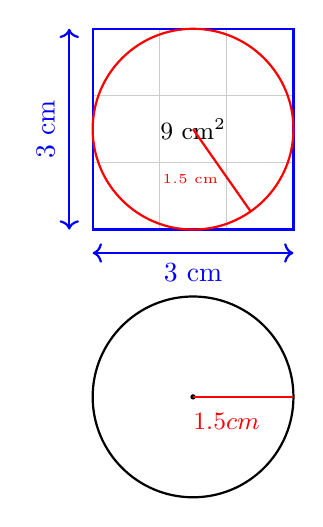
\begin{tikzpicture}[scale=0.85]
  % Grid of squares to illustrate squaring / area idea
  \draw[gray!40, thin] (0,0) grid (3,3);
  \draw[thick, blue] (0,0) rectangle (3,3);
  \draw[blue, thick, <->] (0,-0.35) -- (3,-0.35);
  \node[blue] at (1.5,-0.65) {$3$ cm};
  \draw[blue, thick, <->] (-0.35,0) -- (-0.35,3);
  \node[blue, rotate=90] at (-0.7,1.5) {$3$ cm};
  \node at (1.5,1.5) {\small $9$ cm$^2$};

  % Small circle below for context
  \draw[thick] (1.5,-2.5) circle (1.5cm);
  \fill (1.5,-2.5) circle (0.04);
  \draw[red, thick] (1.5,-2.5) -- ++(0:1.5);
  \node[red, below] at (2,-2.6) {\small $1.5cm$};

% --- Q9 answer: the r = 1.5 cm circle drawn inside the 3 cm square ---
\draw[ans] (1.5,1.5) circle (1.5cm);
\draw[ans] (1.5,1.5) -- ++(-55:1.5);
\node[anslab, left] at (2.02,0.76) {$1.5$ cm};
\end{tikzpicture}
\end{center}

\column{0.65\textwidth}
\small
\begin{enumerate}
  \begin{multicols}{2}
    \item $4 \times 4 = \ashowq{16}$
    \item $7 \times 7 = \ashowq{49}$
  \end{multicols}
  \begin{multicols}{2}
    \item $10^2 = \ashowq{100}$
    \item $3^2 = \ashowq{9}$
  \end{multicols}
  \item $2 \times 6$ and $6^2$ --- are these the same? \ashow{No: $12\neq 36$.}
  \begin{multicols}{2}
  \item $3.14 \times 9=\ablank{28.26}$
  \item $3.14 \times 25=\ablank{78.5}$
  \end{multicols}
\end{enumerate}
\vspace{-1em}
\begin{enumerate}
  \setcounter{enumi}{6}
  \item A circle has \textbf{diameter} $14$ cm. Find: \newline{} (a) the radius \ablank{7\,\text{cm}} \newline{} (b) the circumference \ablank{43.96\,\text{cm}}. ($\pi \approx 3.14$)
  \item A circle has \textbf{radius} $5$ cm. What is the circumference? \ablank{31.4\,\text{cm}}
  \item The square has side $3$ cm and area $9$ cm$^2$. A circle has radius $1.5$ cm. Is the circle's area more or less than $9$ cm$^2$? \ashow{Less: $\pi(1.5)^2 \approx 7.07$ cm$^2$.}
\end{enumerate}

\end{columns}
\end{frame}
\begin{frame}<1>{Starter}

\vspace{-2em}

\begin{columns}

\column{0.35\textwidth}
\begin{center}
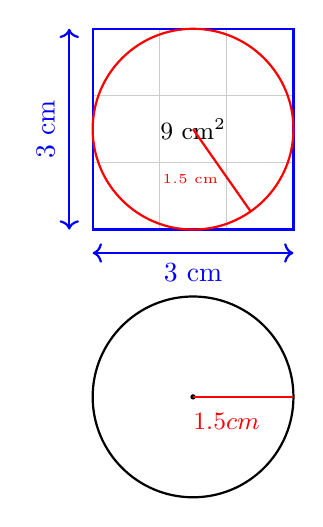
\begin{tikzpicture}[scale=0.85]
  % Grid of squares to illustrate squaring / area idea
  \draw[gray!40, thin] (0,0) grid (3,3);
  \draw[thick, blue] (0,0) rectangle (3,3);
  \draw[blue, thick, <->] (0,-0.35) -- (3,-0.35);
  \node[blue] at (1.5,-0.65) {$3$ cm};
  \draw[blue, thick, <->] (-0.35,0) -- (-0.35,3);
  \node[blue, rotate=90] at (-0.7,1.5) {$3$ cm};
  \node at (1.5,1.5) {\small $9$ cm$^2$};

  % Small circle below for context
  \draw[thick] (1.5,-2.5) circle (1.5cm);
  \fill (1.5,-2.5) circle (0.04);
  \draw[red, thick] (1.5,-2.5) -- ++(0:1.5);
  \node[red, below] at (2,-2.6) {\small $1.5cm$};

% --- Q9 answer: the r = 1.5 cm circle drawn inside the 3 cm square ---
\draw[ans] (1.5,1.5) circle (1.5cm);
\draw[ans] (1.5,1.5) -- ++(-55:1.5);
\node[anslab, left] at (2.02,0.76) {$1.5$ cm};
\end{tikzpicture}
\end{center}

\column{0.65\textwidth}
\small
\begin{enumerate}
  \begin{multicols}{2}
    \item $4 \times 4 = \ashowq{16}$
    \item $7 \times 7 = \ashowq{49}$
  \end{multicols}
  \begin{multicols}{2}
    \item $10^2 = \ashowq{100}$
    \item $3^2 = \ashowq{9}$
  \end{multicols}
  \item $2 \times 6$ and $6^2$ --- are these the same? \ashow{No: $12\neq 36$.}
  \begin{multicols}{2}
  \item $3.14 \times 9=\ablank{28.26}$
  \item $3.14 \times 25=\ablank{78.5}$
  \end{multicols}
\end{enumerate}
\vspace{-1em}
\begin{enumerate}
  \setcounter{enumi}{6}
  \item A circle has \textbf{diameter} $14$ cm. Find: \newline{} (a) the radius \ablank{7\,\text{cm}} \newline{} (b) the circumference \ablank{43.96\,\text{cm}}. ($\pi \approx 3.14$)
  \item A circle has \textbf{radius} $5$ cm. What is the circumference? \ablank{31.4\,\text{cm}}
  \item The square has side $3$ cm and area $9$ cm$^2$. A circle has radius $1.5$ cm. Is the circle's area more or less than $9$ cm$^2$? \ashow{Less: $\pi(1.5)^2 \approx 7.07$ cm$^2$.}
\end{enumerate}

\end{columns}
\end{frame}
\begin{frame}<1>{Starter}

\vspace{-2em}

\begin{columns}

\column{0.35\textwidth}
\begin{center}
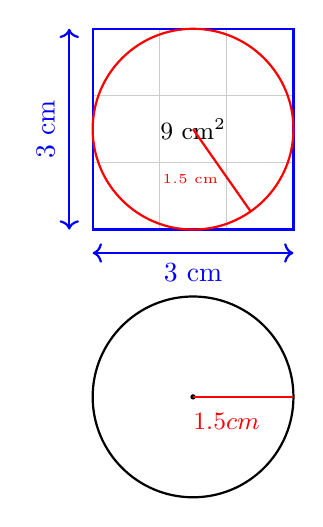
\begin{tikzpicture}[scale=0.85]
  % Grid of squares to illustrate squaring / area idea
  \draw[gray!40, thin] (0,0) grid (3,3);
  \draw[thick, blue] (0,0) rectangle (3,3);
  \draw[blue, thick, <->] (0,-0.35) -- (3,-0.35);
  \node[blue] at (1.5,-0.65) {$3$ cm};
  \draw[blue, thick, <->] (-0.35,0) -- (-0.35,3);
  \node[blue, rotate=90] at (-0.7,1.5) {$3$ cm};
  \node at (1.5,1.5) {\small $9$ cm$^2$};

  % Small circle below for context
  \draw[thick] (1.5,-2.5) circle (1.5cm);
  \fill (1.5,-2.5) circle (0.04);
  \draw[red, thick] (1.5,-2.5) -- ++(0:1.5);
  \node[red, below] at (2,-2.6) {\small $1.5cm$};

% --- Q9 answer: the r = 1.5 cm circle drawn inside the 3 cm square ---
\draw[ans] (1.5,1.5) circle (1.5cm);
\draw[ans] (1.5,1.5) -- ++(-55:1.5);
\node[anslab, left] at (2.02,0.76) {$1.5$ cm};
\end{tikzpicture}
\end{center}

\column{0.65\textwidth}
\small
\begin{enumerate}
  \begin{multicols}{2}
    \item $4 \times 4 = \ashowq{16}$
    \item $7 \times 7 = \ashowq{49}$
  \end{multicols}
  \begin{multicols}{2}
    \item $10^2 = \ashowq{100}$
    \item $3^2 = \ashowq{9}$
  \end{multicols}
  \item $2 \times 6$ and $6^2$ --- are these the same? \ashow{No: $12\neq 36$.}
  \begin{multicols}{2}
  \item $3.14 \times 9=\ablank{28.26}$
  \item $3.14 \times 25=\ablank{78.5}$
  \end{multicols}
\end{enumerate}
\vspace{-1em}
\begin{enumerate}
  \setcounter{enumi}{6}
  \item A circle has \textbf{diameter} $14$ cm. Find: \newline{} (a) the radius \ablank{7\,\text{cm}} \newline{} (b) the circumference \ablank{43.96\,\text{cm}}. ($\pi \approx 3.14$)
  \item A circle has \textbf{radius} $5$ cm. What is the circumference? \ablank{31.4\,\text{cm}}
  \item The square has side $3$ cm and area $9$ cm$^2$. A circle has radius $1.5$ cm. Is the circle's area more or less than $9$ cm$^2$? \ashow{Less: $\pi(1.5)^2 \approx 7.07$ cm$^2$.}
\end{enumerate}

\end{columns}
\end{frame}
\begin{frame}<1>{Starter}

\vspace{-2em}

\begin{columns}

\column{0.35\textwidth}
\begin{center}
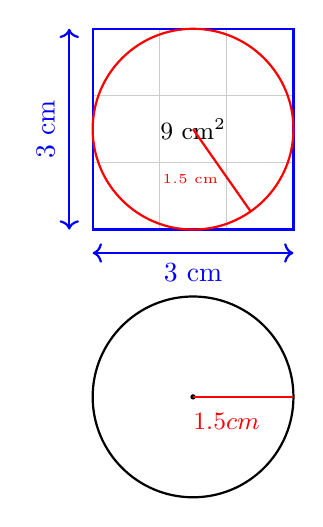
\begin{tikzpicture}[scale=0.85]
  % Grid of squares to illustrate squaring / area idea
  \draw[gray!40, thin] (0,0) grid (3,3);
  \draw[thick, blue] (0,0) rectangle (3,3);
  \draw[blue, thick, <->] (0,-0.35) -- (3,-0.35);
  \node[blue] at (1.5,-0.65) {$3$ cm};
  \draw[blue, thick, <->] (-0.35,0) -- (-0.35,3);
  \node[blue, rotate=90] at (-0.7,1.5) {$3$ cm};
  \node at (1.5,1.5) {\small $9$ cm$^2$};

  % Small circle below for context
  \draw[thick] (1.5,-2.5) circle (1.5cm);
  \fill (1.5,-2.5) circle (0.04);
  \draw[red, thick] (1.5,-2.5) -- ++(0:1.5);
  \node[red, below] at (2,-2.6) {\small $1.5cm$};

% --- Q9 answer: the r = 1.5 cm circle drawn inside the 3 cm square ---
\draw[ans] (1.5,1.5) circle (1.5cm);
\draw[ans] (1.5,1.5) -- ++(-55:1.5);
\node[anslab, left] at (2.02,0.76) {$1.5$ cm};
\end{tikzpicture}
\end{center}

\column{0.65\textwidth}
\small
\begin{enumerate}
  \begin{multicols}{2}
    \item $4 \times 4 = \ashowq{16}$
    \item $7 \times 7 = \ashowq{49}$
  \end{multicols}
  \begin{multicols}{2}
    \item $10^2 = \ashowq{100}$
    \item $3^2 = \ashowq{9}$
  \end{multicols}
  \item $2 \times 6$ and $6^2$ --- are these the same? \ashow{No: $12\neq 36$.}
  \begin{multicols}{2}
  \item $3.14 \times 9=\ablank{28.26}$
  \item $3.14 \times 25=\ablank{78.5}$
  \end{multicols}
\end{enumerate}
\vspace{-1em}
\begin{enumerate}
  \setcounter{enumi}{6}
  \item A circle has \textbf{diameter} $14$ cm. Find: \newline{} (a) the radius \ablank{7\,\text{cm}} \newline{} (b) the circumference \ablank{43.96\,\text{cm}}. ($\pi \approx 3.14$)
  \item A circle has \textbf{radius} $5$ cm. What is the circumference? \ablank{31.4\,\text{cm}}
  \item The square has side $3$ cm and area $9$ cm$^2$. A circle has radius $1.5$ cm. Is the circle's area more or less than $9$ cm$^2$? \ashow{Less: $\pi(1.5)^2 \approx 7.07$ cm$^2$.}
\end{enumerate}

\end{columns}
\end{frame}

%------------------------------------------------
% SLIDE 2: Retrieval + Radius vs Diameter + Squaring in Context
%------------------------------------------------
\begin{frame}<1>{Starter}

\begin{columns}

\column{0.35\textwidth}
\begin{center}
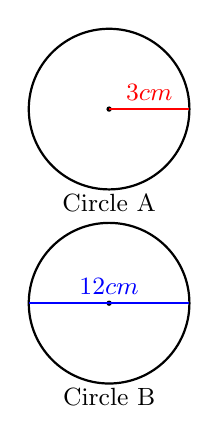
\begin{tikzpicture}[scale=0.85]

  % Circle A — radius labelled
  \draw[thick] (0,2.5) circle (1.2cm);
  \fill (0,2.5) circle (0.04);
  \draw[red, thick] (0,2.5) -- ++(0:1.2);
  \node[red] at (0.6, 2.75) {\small $3cm$};
  \node at (0, 1.1) {\small Circle A};

  % Circle B — diameter labelled
  \draw[thick] (0,-0.4) circle (1.2cm);
  \fill (0,-0.4) circle (0.04);
  \draw[blue, thick] (-1.2,-0.4) -- (1.2,-0.4);
  \node[blue] at (0,-0.15) {\small $12cm$};
  \node at (0,-1.8) {\small Circle B};

\end{tikzpicture}
\end{center}

\column{0.65\textwidth}
\small
\begin{enumerate}
  \begin{multicols}{2}
    \item Halve $12$ cm \ablank{6\,\text{cm}}
    \item Halve $9.4$ cm \ablank{4.7\,\text{cm}}
  \end{multicols}
  \begin{multicols}{2}
    \item $6^2 = \ashowq{36}$
    \item $1.5^2 = \ashowq{2.25}$
  \item $3 \times 4^2=\ablank{48}$
  \item True or false? $\pi \times (2r) = 2 \times \pi \times r$ \ashow{True}
  \end{multicols}
\end{enumerate}
\vspace{-2em}
\begin{enumerate}
  \setcounter{enumi}{6}
  \item Consider circle A \newline{} (a) What is the circumference? \ablank{18.84\,\text{cm}} \newline{} (b) What is the area? \ablank{$28.26\,\text{cm}^2$}
  \item Consider circle B \newline{} (a) What is the circumference? \ablank{37.68\,\text{cm}} \newline{} (b) What is the area? \ablank{$113.04\,\text{cm}^2$}
  \item Is the ratio of the cirumferences of circle's A and B the same as the ratio of the areas? \ashow{No: $1:2$ vs $1:4$.}
\end{enumerate}

\end{columns}
\end{frame}
\begin{frame}<1>{Starter}

\begin{columns}

\column{0.35\textwidth}
\begin{center}
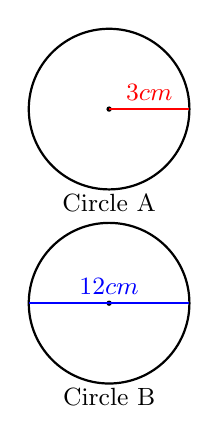
\begin{tikzpicture}[scale=0.85]

  % Circle A — radius labelled
  \draw[thick] (0,2.5) circle (1.2cm);
  \fill (0,2.5) circle (0.04);
  \draw[red, thick] (0,2.5) -- ++(0:1.2);
  \node[red] at (0.6, 2.75) {\small $3cm$};
  \node at (0, 1.1) {\small Circle A};

  % Circle B — diameter labelled
  \draw[thick] (0,-0.4) circle (1.2cm);
  \fill (0,-0.4) circle (0.04);
  \draw[blue, thick] (-1.2,-0.4) -- (1.2,-0.4);
  \node[blue] at (0,-0.15) {\small $12cm$};
  \node at (0,-1.8) {\small Circle B};

\end{tikzpicture}
\end{center}

\column{0.65\textwidth}
\small
\begin{enumerate}
  \begin{multicols}{2}
    \item Halve $12$ cm \ablank{6\,\text{cm}}
    \item Halve $9.4$ cm \ablank{4.7\,\text{cm}}
  \end{multicols}
  \begin{multicols}{2}
    \item $6^2 = \ashowq{36}$
    \item $1.5^2 = \ashowq{2.25}$
  \item $3 \times 4^2=\ablank{48}$
  \item True or false? $\pi \times (2r) = 2 \times \pi \times r$ \ashow{True}
  \end{multicols}
\end{enumerate}
\vspace{-2em}
\begin{enumerate}
  \setcounter{enumi}{6}
  \item Consider circle A \newline{} (a) What is the circumference? \ablank{18.84\,\text{cm}} \newline{} (b) What is the area? \ablank{$28.26\,\text{cm}^2$}
  \item Consider circle B \newline{} (a) What is the circumference? \ablank{37.68\,\text{cm}} \newline{} (b) What is the area? \ablank{$113.04\,\text{cm}^2$}
  \item Is the ratio of the cirumferences of circle's A and B the same as the ratio of the areas? \ashow{No: $1:2$ vs $1:4$.}
\end{enumerate}

\end{columns}
\end{frame}
\begin{frame}<1>{Starter}

\begin{columns}

\column{0.35\textwidth}
\begin{center}
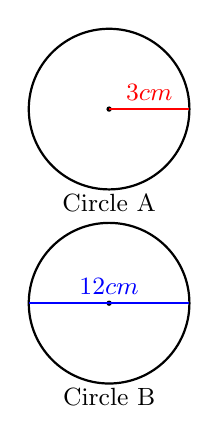
\begin{tikzpicture}[scale=0.85]

  % Circle A — radius labelled
  \draw[thick] (0,2.5) circle (1.2cm);
  \fill (0,2.5) circle (0.04);
  \draw[red, thick] (0,2.5) -- ++(0:1.2);
  \node[red] at (0.6, 2.75) {\small $3cm$};
  \node at (0, 1.1) {\small Circle A};

  % Circle B — diameter labelled
  \draw[thick] (0,-0.4) circle (1.2cm);
  \fill (0,-0.4) circle (0.04);
  \draw[blue, thick] (-1.2,-0.4) -- (1.2,-0.4);
  \node[blue] at (0,-0.15) {\small $12cm$};
  \node at (0,-1.8) {\small Circle B};

\end{tikzpicture}
\end{center}

\column{0.65\textwidth}
\small
\begin{enumerate}
  \begin{multicols}{2}
    \item Halve $12$ cm \ablank{6\,\text{cm}}
    \item Halve $9.4$ cm \ablank{4.7\,\text{cm}}
  \end{multicols}
  \begin{multicols}{2}
    \item $6^2 = \ashowq{36}$
    \item $1.5^2 = \ashowq{2.25}$
  \item $3 \times 4^2=\ablank{48}$
  \item True or false? $\pi \times (2r) = 2 \times \pi \times r$ \ashow{True}
  \end{multicols}
\end{enumerate}
\vspace{-2em}
\begin{enumerate}
  \setcounter{enumi}{6}
  \item Consider circle A \newline{} (a) What is the circumference? \ablank{18.84\,\text{cm}} \newline{} (b) What is the area? \ablank{$28.26\,\text{cm}^2$}
  \item Consider circle B \newline{} (a) What is the circumference? \ablank{37.68\,\text{cm}} \newline{} (b) What is the area? \ablank{$113.04\,\text{cm}^2$}
  \item Is the ratio of the cirumferences of circle's A and B the same as the ratio of the areas? \ashow{No: $1:2$ vs $1:4$.}
\end{enumerate}

\end{columns}
\end{frame}
\begin{frame}<1>{Starter}

\begin{columns}

\column{0.35\textwidth}
\begin{center}
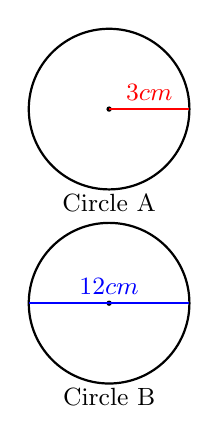
\begin{tikzpicture}[scale=0.85]

  % Circle A — radius labelled
  \draw[thick] (0,2.5) circle (1.2cm);
  \fill (0,2.5) circle (0.04);
  \draw[red, thick] (0,2.5) -- ++(0:1.2);
  \node[red] at (0.6, 2.75) {\small $3cm$};
  \node at (0, 1.1) {\small Circle A};

  % Circle B — diameter labelled
  \draw[thick] (0,-0.4) circle (1.2cm);
  \fill (0,-0.4) circle (0.04);
  \draw[blue, thick] (-1.2,-0.4) -- (1.2,-0.4);
  \node[blue] at (0,-0.15) {\small $12cm$};
  \node at (0,-1.8) {\small Circle B};

\end{tikzpicture}
\end{center}

\column{0.65\textwidth}
\small
\begin{enumerate}
  \begin{multicols}{2}
    \item Halve $12$ cm \ablank{6\,\text{cm}}
    \item Halve $9.4$ cm \ablank{4.7\,\text{cm}}
  \end{multicols}
  \begin{multicols}{2}
    \item $6^2 = \ashowq{36}$
    \item $1.5^2 = \ashowq{2.25}$
  \item $3 \times 4^2=\ablank{48}$
  \item True or false? $\pi \times (2r) = 2 \times \pi \times r$ \ashow{True}
  \end{multicols}
\end{enumerate}
\vspace{-2em}
\begin{enumerate}
  \setcounter{enumi}{6}
  \item Consider circle A \newline{} (a) What is the circumference? \ablank{18.84\,\text{cm}} \newline{} (b) What is the area? \ablank{$28.26\,\text{cm}^2$}
  \item Consider circle B \newline{} (a) What is the circumference? \ablank{37.68\,\text{cm}} \newline{} (b) What is the area? \ablank{$113.04\,\text{cm}^2$}
  \item Is the ratio of the cirumferences of circle's A and B the same as the ratio of the areas? \ashow{No: $1:2$ vs $1:4$.}
\end{enumerate}

\end{columns}
\end{frame}

%------------------------------------------------
% SLIDE 3: Retrieval + Area Intuition + First Explicit Area
%------------------------------------------------
\begin{frame}<1>{Starter}

\vspace{-1em}

\begin{columns}

\column{0.35\textwidth}
\begin{center}
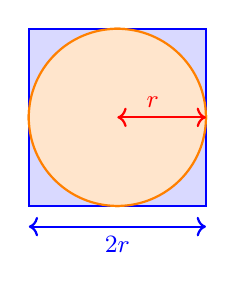
\begin{tikzpicture}[scale=0.75]
  \draw[thick, blue] (0,0) rectangle (3,3);
  \draw[thick, orange] (1.5,1.5) circle (1.5cm);
  \fill (1.5,1.5) circle (0.04);

  % Shade corners to show wasted space
  \begin{scope}
    \clip (0,0) rectangle (3,3);
    \fill[blue!15] (0,0) rectangle (3,3);
    \fill[orange!20] (1.5,1.5) circle (1.5cm);
  \end{scope}
  \draw[thick, blue] (0,0) rectangle (3,3);
  \draw[thick, orange] (1.5,1.5) circle (1.5cm);

  \draw[red, thick, <->] (1.5,1.5) -- ++(0:1.5);
  \node[red] at (2.1,1.75) {\small $r$};
  \draw[blue, thick, <->] (0,-0.35) -- (3,-0.35);
  \node[blue] at (1.5,-0.65) {\small $2r$};

\end{tikzpicture}
\end{center}

\column{0.65\textwidth}
\small
\begin{enumerate}
  \begin{multicols}{2}
    \item $5 \times 5 = \ashowq{25}$
    \item $8^2 = \ashowq{64}$
  \end{multicols}
  \begin{multicols}{2}
    \item $2.5^2 = \ashowq{6.25}$
    \item $3.14 \times 9 = \ablank{28.26}$
  \end{multicols}
  \item Area of a $7$ cm $\times$ $4$ cm rectangle $= \ashowq{28\,\text{cm}^2}$
  \item What fraction of $360^\circ$ is $90^\circ$? \ashow{$\frac{1}{4}$}
\end{enumerate}

\begin{enumerate}
  \setcounter{enumi}{6}
  \item Write an expression for the area of the circle in the picture \ashow{$\pi r^2$}
  \item Write an expression for the area of the shaded blue region in the picture \ashow{$4r^2-\pi r^2$}
  \item If the square has a perimeter of 48cm, what is the area of the shaded blue region? \ashow{$30.96\,\text{cm}^2$}
\end{enumerate}

\end{columns}
\end{frame}
\begin{frame}<1>{Starter}

\vspace{-1em}

\begin{columns}

\column{0.35\textwidth}
\begin{center}
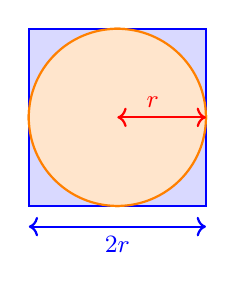
\begin{tikzpicture}[scale=0.75]
  \draw[thick, blue] (0,0) rectangle (3,3);
  \draw[thick, orange] (1.5,1.5) circle (1.5cm);
  \fill (1.5,1.5) circle (0.04);

  % Shade corners to show wasted space
  \begin{scope}
    \clip (0,0) rectangle (3,3);
    \fill[blue!15] (0,0) rectangle (3,3);
    \fill[orange!20] (1.5,1.5) circle (1.5cm);
  \end{scope}
  \draw[thick, blue] (0,0) rectangle (3,3);
  \draw[thick, orange] (1.5,1.5) circle (1.5cm);

  \draw[red, thick, <->] (1.5,1.5) -- ++(0:1.5);
  \node[red] at (2.1,1.75) {\small $r$};
  \draw[blue, thick, <->] (0,-0.35) -- (3,-0.35);
  \node[blue] at (1.5,-0.65) {\small $2r$};

\end{tikzpicture}
\end{center}

\column{0.65\textwidth}
\small
\begin{enumerate}
  \begin{multicols}{2}
    \item $5 \times 5 = \ashowq{25}$
    \item $8^2 = \ashowq{64}$
  \end{multicols}
  \begin{multicols}{2}
    \item $2.5^2 = \ashowq{6.25}$
    \item $3.14 \times 9 = \ablank{28.26}$
  \end{multicols}
  \item Area of a $7$ cm $\times$ $4$ cm rectangle $= \ashowq{28\,\text{cm}^2}$
  \item What fraction of $360^\circ$ is $90^\circ$? \ashow{$\frac{1}{4}$}
\end{enumerate}

\begin{enumerate}
  \setcounter{enumi}{6}
  \item Write an expression for the area of the circle in the picture \ashow{$\pi r^2$}
  \item Write an expression for the area of the shaded blue region in the picture \ashow{$4r^2-\pi r^2$}
  \item If the square has a perimeter of 48cm, what is the area of the shaded blue region? \ashow{$30.96\,\text{cm}^2$}
\end{enumerate}

\end{columns}
\end{frame}
\begin{frame}<1>{Starter}

\vspace{-1em}

\begin{columns}

\column{0.35\textwidth}
\begin{center}
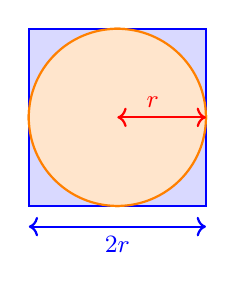
\begin{tikzpicture}[scale=0.75]
  \draw[thick, blue] (0,0) rectangle (3,3);
  \draw[thick, orange] (1.5,1.5) circle (1.5cm);
  \fill (1.5,1.5) circle (0.04);

  % Shade corners to show wasted space
  \begin{scope}
    \clip (0,0) rectangle (3,3);
    \fill[blue!15] (0,0) rectangle (3,3);
    \fill[orange!20] (1.5,1.5) circle (1.5cm);
  \end{scope}
  \draw[thick, blue] (0,0) rectangle (3,3);
  \draw[thick, orange] (1.5,1.5) circle (1.5cm);

  \draw[red, thick, <->] (1.5,1.5) -- ++(0:1.5);
  \node[red] at (2.1,1.75) {\small $r$};
  \draw[blue, thick, <->] (0,-0.35) -- (3,-0.35);
  \node[blue] at (1.5,-0.65) {\small $2r$};

\end{tikzpicture}
\end{center}

\column{0.65\textwidth}
\small
\begin{enumerate}
  \begin{multicols}{2}
    \item $5 \times 5 = \ashowq{25}$
    \item $8^2 = \ashowq{64}$
  \end{multicols}
  \begin{multicols}{2}
    \item $2.5^2 = \ashowq{6.25}$
    \item $3.14 \times 9 = \ablank{28.26}$
  \end{multicols}
  \item Area of a $7$ cm $\times$ $4$ cm rectangle $= \ashowq{28\,\text{cm}^2}$
  \item What fraction of $360^\circ$ is $90^\circ$? \ashow{$\frac{1}{4}$}
\end{enumerate}

\begin{enumerate}
  \setcounter{enumi}{6}
  \item Write an expression for the area of the circle in the picture \ashow{$\pi r^2$}
  \item Write an expression for the area of the shaded blue region in the picture \ashow{$4r^2-\pi r^2$}
  \item If the square has a perimeter of 48cm, what is the area of the shaded blue region? \ashow{$30.96\,\text{cm}^2$}
\end{enumerate}

\end{columns}
\end{frame}
\begin{frame}<1>{Starter}

\vspace{-1em}

\begin{columns}

\column{0.35\textwidth}
\begin{center}
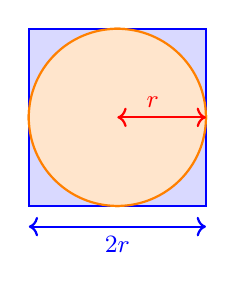
\begin{tikzpicture}[scale=0.75]
  \draw[thick, blue] (0,0) rectangle (3,3);
  \draw[thick, orange] (1.5,1.5) circle (1.5cm);
  \fill (1.5,1.5) circle (0.04);

  % Shade corners to show wasted space
  \begin{scope}
    \clip (0,0) rectangle (3,3);
    \fill[blue!15] (0,0) rectangle (3,3);
    \fill[orange!20] (1.5,1.5) circle (1.5cm);
  \end{scope}
  \draw[thick, blue] (0,0) rectangle (3,3);
  \draw[thick, orange] (1.5,1.5) circle (1.5cm);

  \draw[red, thick, <->] (1.5,1.5) -- ++(0:1.5);
  \node[red] at (2.1,1.75) {\small $r$};
  \draw[blue, thick, <->] (0,-0.35) -- (3,-0.35);
  \node[blue] at (1.5,-0.65) {\small $2r$};

\end{tikzpicture}
\end{center}

\column{0.65\textwidth}
\small
\begin{enumerate}
  \begin{multicols}{2}
    \item $5 \times 5 = \ashowq{25}$
    \item $8^2 = \ashowq{64}$
  \end{multicols}
  \begin{multicols}{2}
    \item $2.5^2 = \ashowq{6.25}$
    \item $3.14 \times 9 = \ablank{28.26}$
  \end{multicols}
  \item Area of a $7$ cm $\times$ $4$ cm rectangle $= \ashowq{28\,\text{cm}^2}$
  \item What fraction of $360^\circ$ is $90^\circ$? \ashow{$\frac{1}{4}$}
\end{enumerate}

\begin{enumerate}
  \setcounter{enumi}{6}
  \item Write an expression for the area of the circle in the picture \ashow{$\pi r^2$}
  \item Write an expression for the area of the shaded blue region in the picture \ashow{$4r^2-\pi r^2$}
  \item If the square has a perimeter of 48cm, what is the area of the shaded blue region? \ashow{$30.96\,\text{cm}^2$}
\end{enumerate}

\end{columns}
\end{frame}

%------------------------------------------------
% SLIDE 4: Full Retrieval + Fluency with Area + Spot the Error
%------------------------------------------------
\begin{frame}<1>{Starter}

\vspace{-1em}

\begin{columns}

\column{0.35\textwidth}
\begin{center}
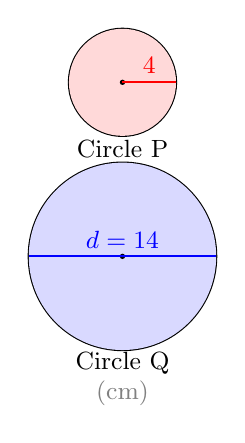
\begin{tikzpicture}[scale=0.85]

  % Two circles for comparison
  \draw[thick] (0, 2.2) circle (0.8cm);
  \fill[red!15] (0,2.2) circle (0.8cm);
  \fill (0,2.2) circle (0.04);
  \draw[red, thick] (0,2.2) -- ++(0:0.8);
  \node[red] at (0.4, 2.45) {\small $4$};
  \node at (0, 1.2) {\small Circle P};

  \draw[thick] (0,-0.4) circle (1.4cm);
  \fill[blue!15] (0,-0.4) circle (1.4cm);
  \fill (0,-0.4) circle (0.04);
  \draw[blue, thick] (-1.4,-0.4) -- (1.4,-0.4);
  \node[blue] at (0,-0.15) {\small $d=14$};
  \node at (0,-2.0) {\small Circle Q};

  \node[gray] at (0,-2.45) {\small (cm)};

\end{tikzpicture}
\end{center}

\column{0.65\textwidth}
\small
\begin{enumerate}
  \begin{multicols}{2}
    \item $9^2 = \ashowq{81}$
    \item $3.5^2 = \ashowq{12.25}$
  \end{multicols}
  \begin{multicols}{2}
    \item $3.14 \times 16$ \ashow{$=50.24$}
    \item $3.14 \times 49$ \ashow{$=153.86$}
  \end{multicols}
  \item Halve $14$ cm. \quad Then square your answer. \ashow{$7$ cm, so $49\,\text{cm}^2$}
  \item A square has area $64$ cm$^2$. What is its side length \ashowq{$8$ cm}
\end{enumerate}

\begin{enumerate}
  \setcounter{enumi}{6}
  \item \textbf{Spot the mistake:} \textit{``Circle Q has diameter $14$ cm, so its area is $\pi \times 14^2 \approx 615$ cm$^2$.''} What error was made? Write the correct solution. \ashow{Used diameter not radius: $\pi \times 7^2 \approx 153.86\,\text{cm}^2$.}
  \item \textbf{Circle P}, radius $4$ cm. Find: (a) the area \ablank{$50.24\,\text{cm}^2$} \quad (b) the circumference \ablank{25.12\,\text{cm}}.
  \item \textbf{Circle Q}, diameter $14$ cm. Find: (a) the area \ablank{$153.86\,\text{cm}^2$} \quad (b) the circumference \ablank{43.96\,\text{cm}}.
  \item Which has the greater area, P or Q? By approximately how many cm$^2$? \ashow{Q, by approximately $103.62\,\text{cm}^2$.}
\end{enumerate}

\end{columns}
\end{frame}
\begin{frame}<1>{Starter}

\vspace{-1em}

\begin{columns}

\column{0.35\textwidth}
\begin{center}
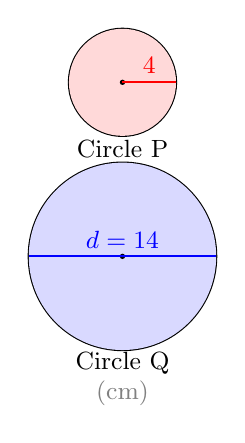
\begin{tikzpicture}[scale=0.85]

  % Two circles for comparison
  \draw[thick] (0, 2.2) circle (0.8cm);
  \fill[red!15] (0,2.2) circle (0.8cm);
  \fill (0,2.2) circle (0.04);
  \draw[red, thick] (0,2.2) -- ++(0:0.8);
  \node[red] at (0.4, 2.45) {\small $4$};
  \node at (0, 1.2) {\small Circle P};

  \draw[thick] (0,-0.4) circle (1.4cm);
  \fill[blue!15] (0,-0.4) circle (1.4cm);
  \fill (0,-0.4) circle (0.04);
  \draw[blue, thick] (-1.4,-0.4) -- (1.4,-0.4);
  \node[blue] at (0,-0.15) {\small $d=14$};
  \node at (0,-2.0) {\small Circle Q};

  \node[gray] at (0,-2.45) {\small (cm)};

\end{tikzpicture}
\end{center}

\column{0.65\textwidth}
\small
\begin{enumerate}
  \begin{multicols}{2}
    \item $9^2 = \ashowq{81}$
    \item $3.5^2 = \ashowq{12.25}$
  \end{multicols}
  \begin{multicols}{2}
    \item $3.14 \times 16$ \ashow{$=50.24$}
    \item $3.14 \times 49$ \ashow{$=153.86$}
  \end{multicols}
  \item Halve $14$ cm. \quad Then square your answer. \ashow{$7$ cm, so $49\,\text{cm}^2$}
  \item A square has area $64$ cm$^2$. What is its side length \ashowq{$8$ cm}
\end{enumerate}

\begin{enumerate}
  \setcounter{enumi}{6}
  \item \textbf{Spot the mistake:} \textit{``Circle Q has diameter $14$ cm, so its area is $\pi \times 14^2 \approx 615$ cm$^2$.''} What error was made? Write the correct solution. \ashow{Used diameter not radius: $\pi \times 7^2 \approx 153.86\,\text{cm}^2$.}
  \item \textbf{Circle P}, radius $4$ cm. Find: (a) the area \ablank{$50.24\,\text{cm}^2$} \quad (b) the circumference \ablank{25.12\,\text{cm}}.
  \item \textbf{Circle Q}, diameter $14$ cm. Find: (a) the area \ablank{$153.86\,\text{cm}^2$} \quad (b) the circumference \ablank{43.96\,\text{cm}}.
  \item Which has the greater area, P or Q? By approximately how many cm$^2$? \ashow{Q, by approximately $103.62\,\text{cm}^2$.}
\end{enumerate}

\end{columns}
\end{frame}
\begin{frame}<1>{Starter}

\vspace{-1em}

\begin{columns}

\column{0.35\textwidth}
\begin{center}
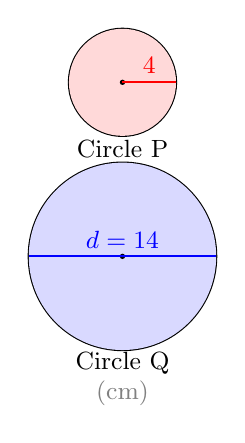
\begin{tikzpicture}[scale=0.85]

  % Two circles for comparison
  \draw[thick] (0, 2.2) circle (0.8cm);
  \fill[red!15] (0,2.2) circle (0.8cm);
  \fill (0,2.2) circle (0.04);
  \draw[red, thick] (0,2.2) -- ++(0:0.8);
  \node[red] at (0.4, 2.45) {\small $4$};
  \node at (0, 1.2) {\small Circle P};

  \draw[thick] (0,-0.4) circle (1.4cm);
  \fill[blue!15] (0,-0.4) circle (1.4cm);
  \fill (0,-0.4) circle (0.04);
  \draw[blue, thick] (-1.4,-0.4) -- (1.4,-0.4);
  \node[blue] at (0,-0.15) {\small $d=14$};
  \node at (0,-2.0) {\small Circle Q};

  \node[gray] at (0,-2.45) {\small (cm)};

\end{tikzpicture}
\end{center}

\column{0.65\textwidth}
\small
\begin{enumerate}
  \begin{multicols}{2}
    \item $9^2 = \ashowq{81}$
    \item $3.5^2 = \ashowq{12.25}$
  \end{multicols}
  \begin{multicols}{2}
    \item $3.14 \times 16$ \ashow{$=50.24$}
    \item $3.14 \times 49$ \ashow{$=153.86$}
  \end{multicols}
  \item Halve $14$ cm. \quad Then square your answer. \ashow{$7$ cm, so $49\,\text{cm}^2$}
  \item A square has area $64$ cm$^2$. What is its side length \ashowq{$8$ cm}
\end{enumerate}

\begin{enumerate}
  \setcounter{enumi}{6}
  \item \textbf{Spot the mistake:} \textit{``Circle Q has diameter $14$ cm, so its area is $\pi \times 14^2 \approx 615$ cm$^2$.''} What error was made? Write the correct solution. \ashow{Used diameter not radius: $\pi \times 7^2 \approx 153.86\,\text{cm}^2$.}
  \item \textbf{Circle P}, radius $4$ cm. Find: (a) the area \ablank{$50.24\,\text{cm}^2$} \quad (b) the circumference \ablank{25.12\,\text{cm}}.
  \item \textbf{Circle Q}, diameter $14$ cm. Find: (a) the area \ablank{$153.86\,\text{cm}^2$} \quad (b) the circumference \ablank{43.96\,\text{cm}}.
  \item Which has the greater area, P or Q? By approximately how many cm$^2$? \ashow{Q, by approximately $103.62\,\text{cm}^2$.}
\end{enumerate}

\end{columns}
\end{frame}
\begin{frame}<1>{Starter}

\vspace{-1em}

\begin{columns}

\column{0.35\textwidth}
\begin{center}
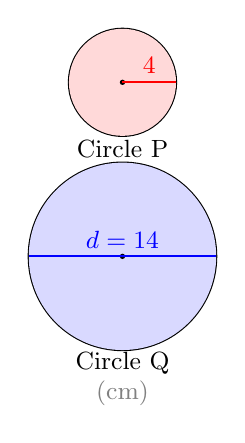
\begin{tikzpicture}[scale=0.85]

  % Two circles for comparison
  \draw[thick] (0, 2.2) circle (0.8cm);
  \fill[red!15] (0,2.2) circle (0.8cm);
  \fill (0,2.2) circle (0.04);
  \draw[red, thick] (0,2.2) -- ++(0:0.8);
  \node[red] at (0.4, 2.45) {\small $4$};
  \node at (0, 1.2) {\small Circle P};

  \draw[thick] (0,-0.4) circle (1.4cm);
  \fill[blue!15] (0,-0.4) circle (1.4cm);
  \fill (0,-0.4) circle (0.04);
  \draw[blue, thick] (-1.4,-0.4) -- (1.4,-0.4);
  \node[blue] at (0,-0.15) {\small $d=14$};
  \node at (0,-2.0) {\small Circle Q};

  \node[gray] at (0,-2.45) {\small (cm)};

\end{tikzpicture}
\end{center}

\column{0.65\textwidth}
\small
\begin{enumerate}
  \begin{multicols}{2}
    \item $9^2 = \ashowq{81}$
    \item $3.5^2 = \ashowq{12.25}$
  \end{multicols}
  \begin{multicols}{2}
    \item $3.14 \times 16$ \ashow{$=50.24$}
    \item $3.14 \times 49$ \ashow{$=153.86$}
  \end{multicols}
  \item Halve $14$ cm. \quad Then square your answer. \ashow{$7$ cm, so $49\,\text{cm}^2$}
  \item A square has area $64$ cm$^2$. What is its side length \ashowq{$8$ cm}
\end{enumerate}

\begin{enumerate}
  \setcounter{enumi}{6}
  \item \textbf{Spot the mistake:} \textit{``Circle Q has diameter $14$ cm, so its area is $\pi \times 14^2 \approx 615$ cm$^2$.''} What error was made? Write the correct solution. \ashow{Used diameter not radius: $\pi \times 7^2 \approx 153.86\,\text{cm}^2$.}
  \item \textbf{Circle P}, radius $4$ cm. Find: (a) the area \ablank{$50.24\,\text{cm}^2$} \quad (b) the circumference \ablank{25.12\,\text{cm}}.
  \item \textbf{Circle Q}, diameter $14$ cm. Find: (a) the area \ablank{$153.86\,\text{cm}^2$} \quad (b) the circumference \ablank{43.96\,\text{cm}}.
  \item Which has the greater area, P or Q? By approximately how many cm$^2$? \ashow{Q, by approximately $103.62\,\text{cm}^2$.}
\end{enumerate}

\end{columns}
\end{frame}

\end{document}